\documentclass[]{article}
% used packages
\usepackage[german]{babel}   % enables umlaute
\usepackage[utf8]{inputenc}  % set encoding to utf8 otherwise no umlaute
\usepackage{graphicx}        % for including graphics
\usepackage[hidelinks]{hyperref}        % for using hyperlinks in the document
\usepackage{tabularx}        % for extending tabluar
\usepackage{multirow}        % for rowspan in tabularx
\usepackage{ltablex}         % tables over multiple pages
\usepackage{textcmds}        % for quote support
\usepackage{pdfpages}        % for pdf include
\usepackage{caption}
\usepackage{minted}
\usepackage{listings}
\usepackage[left=1.0in, right=1.0in, top=1.0in, bottom=1.0in]{geometry} % for custom page layout

% Title Page
\title{Raspberry PI Security Application}
\author{Thonas Herzog, Philipp Wurm}


\newcommand{\imageDir}{../images}
\newcommand{\srcDir}{../example-src}
\newcommand{\dockerTestDir}{../../java/testsuite/client/src/main/resources/docker}
\newcommand{\dockerRPIDir}{../../host/docker}
\renewcommand\listingscaption{Quelltext}

\newenvironment{code}{\captionsetup{type=listing}}{}

\newmintedfile[yamlFile]{yaml}{
	linenos=true, 
	frame=single, 
	breaklines=true, 
	tabsize=2,
	numbersep=5pt,
	xleftmargin=10pt,
	baselinestretch=1,
	fontsize=\footnotesize
}

\begin{document}
\maketitle

\begin{abstract}
\end{abstract}

\section{Einleitung}
Diese Dokument stellt die Dokumentation des Projekts \emph{Raspberry PI Security Application}, in weiterer Folge \emph{RPISec} genannt, dar, welches für die Lehrveranstaltung \emph{Mobile und ubiquitäre Systeme} realisiert wurde. In diesem Projekt wird eine Heimsicherheitsanwendung mit einem \emph{Raspberry PI 3 Model B}, \emph{Docker} und \emph{Spring Boot Microservice} umgesetzt, das bei einem Sicherheitsverstoß in der Lage ist, bekannte mobile Endgeräte von registrierten Benutzern über diesen Sicherheitsverstoß zu informieren. 

\subsection{Problemdarstellung}
Dieser Abschnitt behandelt die Problemdarstellung, welche die Grundlage für das umzusetzende Projekt \emph{RPISec} ist. Bei einem Auslösen des am \emph{Raspberry PI} angeschlossenen Bewegungssensors sollen alle am System registrierten Benutzer über ihre mobilen Endgeräte wie Handy oder Tablet über den Vorfall informiert werden, sowie die Möglichkeit haben ein Bild zu erhalten, welches den Sicherheitsbereich zum Zeitpunkt des Sicherheitsverstoßes zeigt. 
\newline
\newline
Da es sich um eine Sicherheitsanwendung handelt, soll die Benutzerverwaltung sowie die Authentifizierung \emph{In-House} gehalten werden, also die Sicherheitsanwendung selbst soll in der Lage sein die Benutzer zu verwalten und die Authentifizierungen der Benutzer durchzuführen. Da sich die mobilen Endgeräte in irgendwelchen Netzen ans Internet anbinden können, wie zum Beispiel über einen Mobilfunkanbieter, Internetanbieter oder öffentlichen \emph{Hot-Spot}, wird ein \emph{Messaging} Dienst benötigt, über den die mobilen Endgeräte erreicht werden können. Dieser \emph{Messaging} Dienst muss es erlauben, dass die Benutzerverwaltung extern erfolgen kann, da wir diesen \emph{Messaging} Dienst nicht vertrauen wollen und daher den \emph{Messaging} Dienst auch nicht die Benutzerverwaltung überlassen wollen. Ebenso wird ein online Speichermedium benötigt, dass alle Bilder speichert, damit die registrierten Benutzer jederzeit darauf zugreifen können.


\subsection{Funktionsweise}
Dieser Abschnitt behandelt die Funktionsweise der Applikation \emph{RPISec}. Die Abbildung \ref{fig:image-system-structure} zeigt den Systemaufbau der \emph{RPISec} Applikation mit der involvierten Hardware und \emph{Cloud} Dienst. 
\begin{figure}[h]
	\centering
	\includegraphics[scale=0.7]{\imageDir/Infrastructure.jpg}
	\caption{Systemaufbau der \emph{RPISec} Applikation}
	\label{fig:image-system-structure}
\end{figure}
\ \newpage

\subsubsection{Zugangsverifikation}
Beim Start des Systems wird vom Authentifizierungsservice \emph{(Auth-Service)} ein Administrator Benutzer erstellt, wenn dieser nicht bereits existiert. Ein neu angelegter Benutzer wird über eine E-Mail dazu aufgefordert, seinen Zugang zu aktivieren, in dem er ein Password vergibt. Im Idealfall würde die Zugangsverifikation nur im Heimnetz möglich.
\begin{figure}[h]
	\centering
	\includegraphics[scale=0.5]{\imageDir/view-verify-account.JPG}
	\caption{Zugangsaktivierung}
	\label{fig:image-veriy-account}
\end{figure}
\begin{figure}[h]
	\centering
	\includegraphics[scale=0.5]{\imageDir/view-verified-account.JPG}
	\caption{Bestätigung der Aktivierung}
	\label{fig:image-veriied-account}
\end{figure}

\subsubsection{\emph{Client Login}}
Die Abbildung \ref{fig:image-sequence-client-login} zeigt das Sequenzdiagramm, welches den Ablauf eines Logins eines Benutzers über einen mobilen \emph{Client} beschreibt.
\begin{figure}[h]
	\centering
	\includegraphics[scale=0.55]{\imageDir/sequence-client-login.jpg}
	\caption{Sequenzdiagramm des Logins über einen mobilen \emph{Client}}
	\label{fig:image-sequence-client-login}
\end{figure}
\ \newline
Im Zuge des Logins wird der mobile \emph{Client} am \emph{(Auth-Service)}, der die Authentifizierung durchführt, und am Applikationsservice \emph{App-Service} registriert. Der \emph{Auth-Service} erstellt bei jedem Login einen neuen \emph{OAuth2-Client} und löscht gegebenenfalls einen bestehenden  \emph{OAuth2-Client} für den mobilen \emph{Client}. Das erstellen eines \emph{OAuth2-Clients} wird durchgeführt, da mit der \emph{Client}-Applikation keine \emph{Oauth2-Client} Zugangsdaten an die mobilen \emph{Clients} mit ausgeliefert werden sollen.
\newline
\newline
Dem mobilen \emph{Client} wird bei einem Login ein \emph{Firebase} Authentifizierungstoken übermittelt, mit dem sich der \emph{Client} and \emph{Firebase} anmelden kann. Nachdem Login eines mobilen \emph{Clients} auf \emph{Firebase} holt sich der mobile \emph{Client} seine eindeutige \emph{FCM} Id in Form eines Tokens, der am \emph{Auth-Service} registriert wird, der wiederum den Token am \emph{App-Service} registriert, damit dieser in der Lage ist Nachrichten an die angemeldeten mobilen \emph{Clients} zu versenden.  

\subsubsection{Sicherheitsverstoß melden}
\begin{figure}[h]
	\centering
	\includegraphics[scale=0.55]{\imageDir/sequence-incident.jpg}
	\caption{Sequenzdiagramm des Behandelns eines Sicherheitsverstoßes}
	\label{fig:image-sequence-incident}
\end{figure}
\ \newline
Die Abbildung \ref{fig:image-sequence-incident} zeigt das Sequenzdiagramm für das Behandeln eines Sicherheitsverstoßes, der von der Sensorapplikation erkannt und dem Applikationsservice mitgeteilt wird. Der Sicherheitsverstoß wird über \emph{Firebase} an die mobilen \emph{Clients} gemeldet, wobei einerseits eine \emph{Firebase Cloud Message (FCM)} an die mobilen \emph{Clients} versendet wird, sowie das gemachte Bild in einer \emph{Firebase} JSON-Datenbank den mobilen \emph{Clients} zum Download zur Verfügung gestellt wird. Die Benutzer können jederzeit auf die JSON-Datenbank zugreifen und sich die Bilder auf ihren jeweiligen mobilen \emph{Client} herunterladen. 
\newline
\newline
Der Ansatz einen \emph{Cloud} Dienst zu verwenden sorgt dafür, dass das \emph{RPISec} System entlastet wird, da der Datenfluss und die Netzwerkzugriffe vom System ins Internet sowie umgekehrt minimiert wird. Die Daten müssen nur einmalig in die \emph{Cloud} hochgeladen werden und die Benutzer können jederzeit, beliebig oft und von jedem beliebigen mobilen \emph{Client} darauf zugreifen.
\newpage
 
\subsubsection{\emph{Client} Nachrichtenempfang}
Die Abbildung \ref{fig:image-sequence-client-notification} zeigt den Ablauf einer  Benachrichtigung eines \emph{Client} über den \emph{Firebase Messaging} Dienst.
\begin{figure}[h]
	\centering
	\includegraphics[scale=0.55]{\imageDir/sequence-client-notification.jpg}
	\caption{Sequenzdiagramm der Benachrichtigung eines \emph{Client}}
	\label{fig:image-sequence-client-notification}
\end{figure}
\ \newline
Nachdem das System \emph{RPISec} die mobilen \emph{Clients} via \emph{Firebase Cloud Messages} über einen Sicherheitsverstoß benachrichtigt hat, erhalten die mobilen \emph{Client}-Anwendungen die Nachricht von \emph{Firebase} und zeigen diese an. Nachdem die Benutzer auf die Nachricht geklickt haben, wird eine \emph{Activity} für das Anzeigen der Bilder geöffnet, die alle bereits gespeicherten Bilder und das neu geladene Bild anzeigt. Diese Daten werden von der \emph{Firebase} JSON-Datenbank geladen. 
\section{\emph{Raspberry PI}}
\label{sec:raspberrypi}
Dieser Abschnitt behandelt den Aufbau von \emph{RPISec} und die verwendete Hardware. Für den Testaufbau wurden folgende Hardwarekomponenten verwendet.
\begin{itemize}
	\item Ein \emph{Raspberry PI 3 Model B}\footnote{\url{https://www.raspberrypi.org/products/raspberry-pi-3-model-b/}},
	\item \emph{AZDeliveryCamRasp}\footnote{\url{https://az-delivery.de/products/raspberrykamerav1-3}} und ein
	\item \emph{HC-SR501\footnote{\url{https://www.mpja.com/download/31227sc.pdf}} Bewegungssensor}.
\end{itemize}
\begin{figure}[h]
	\centering
	\includegraphics[scale=0.45]{\imageDir/rpisec-hardware-setup.png}
	\caption{Testaufbau der Applikation}
	\label{fig:image-hardware-setup}
\end{figure}
\ \newline
Die Abbildung \ref{fig:image-hardware-setup} zeigt den verwendeten Testaufbau. Die Kamera wurde über CSI \emph{(Camera-Serial-Interface)}) und der Bewegungssensor über GPIO \emph{(General Purpose Input/Output)} an den \emph{Raspberry PI} angeschlossen.

\subsection{Kamera}
Bei der Kamera handelt es sich um ein eigens für den \emph{Raspberry Pi} entwickeltes Modell und wird direkt an den vorhanden Kamera-Port (CSI) des \emph{Raspberry Pi} 3\footnote{\url{https://en.wikipedia.org/wiki/Raspberry_Pi\#/media/File:Raspberry-Pi-3-Flat-Top.jpg}} angeschlossen. Anschließend muss die Kamera aktiviert werden. Dies geschieht über das, mit den meisten Linux-Distributionen mitgelieferte, Programm \emph{raspi-config\footnote{\url{https://upload.wikimedia.org/wikipedia/commons/e/ed/Raspi-config.png}}}. Dieses Programm wird auch benutzt, um andere Komponenten des \emph{Raspberry Pi} zu konfigurieren.
\newpage
\begin{figure}[h]
	\centering
	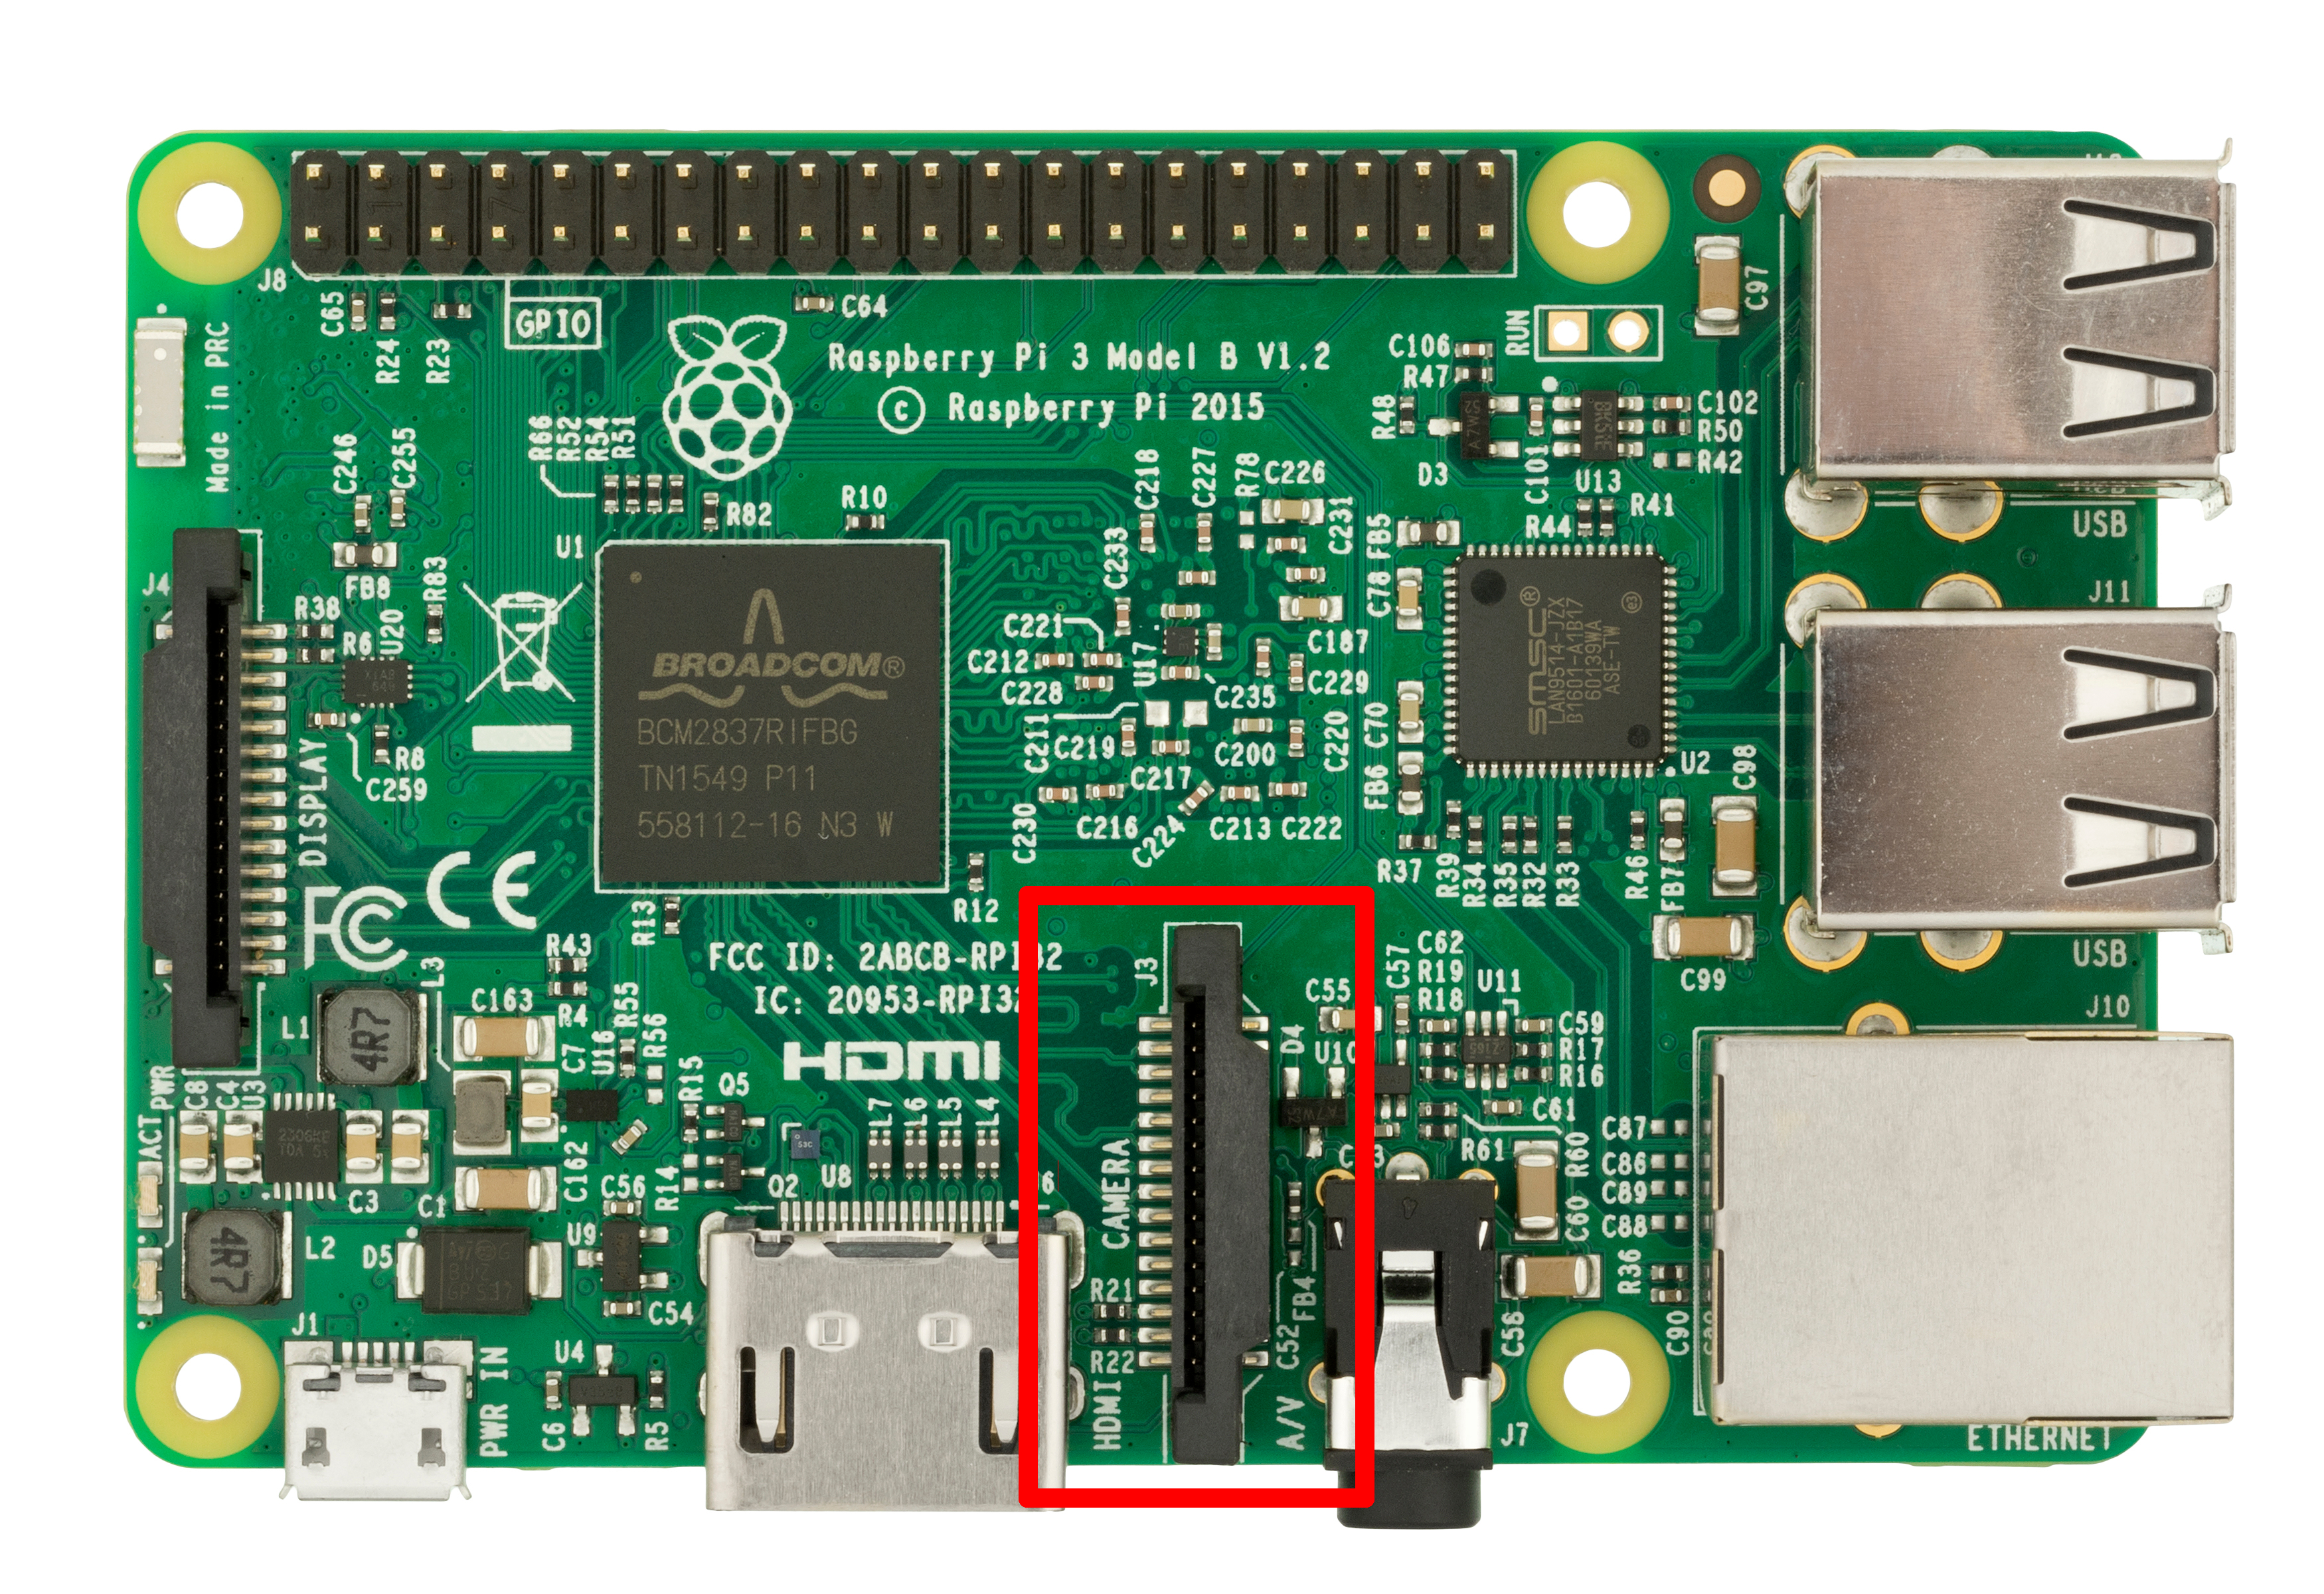
\includegraphics[scale=0.30]{\imageDir/rpi-border-cam.jpg}
	\caption{Raspberry-Pi 3}
	\label{fig:rpi-border-cam}
\end{figure}
\ \newline
Die Abbildung \ref{fig:raspi-config-cam} zeigt die Oberfläche, über welche die Kamera aktiviert werden kann.
\begin{figure}[h]
	\centering
	\includegraphics[scale=0.60]{\imageDir/raspi-config-cam.png}
	%By Onepiece84 (Own work) [CC BY-SA 4.0 (http://creativecommons.org/licenses/by-sa/4.0)], via Wikimedia Commons
	\caption{Raspi-config}
	\label{fig:raspi-config-cam}
\end{figure}
\ \newline
Zur Ansteuerung der Kamera wird das Konsolenprogramm \emph{raspistill} verwendet. Diese kann mit verschiedensten Parametern konfiguriert werden. Als Beispiel:
\begin{minted}{bash}
	raspistill --width 1920 --height 1080 -o test.jpg
\end{minted}
Dies erzeugt ein Bild in der Auflösung 1920 x 1080 Pixel und speichert es unter dem Dateinamen \emph{test.jpg}. \emph{RPISec} wird in \emph{Docker Containern} gehostet und die Anwendung \emph{raspistill} wird in ein \emph{Docker Image} installiert und muss daher nicht am Host installiert werden.
\newpage

\subsection{HC-SR501 Bewegungssensor}
Der HC-SR501 Sensor wird über die \emph{GPIO-Pins} des \emph{Raspberry Pi} angesteuert. Hierbei werden Masse, Stromversorgung und Daten-Pin des HC-SR501 Sensors mit den \emph{GPIO-Pins} verbunden. 

\begin{figure}[h]
	\centering
	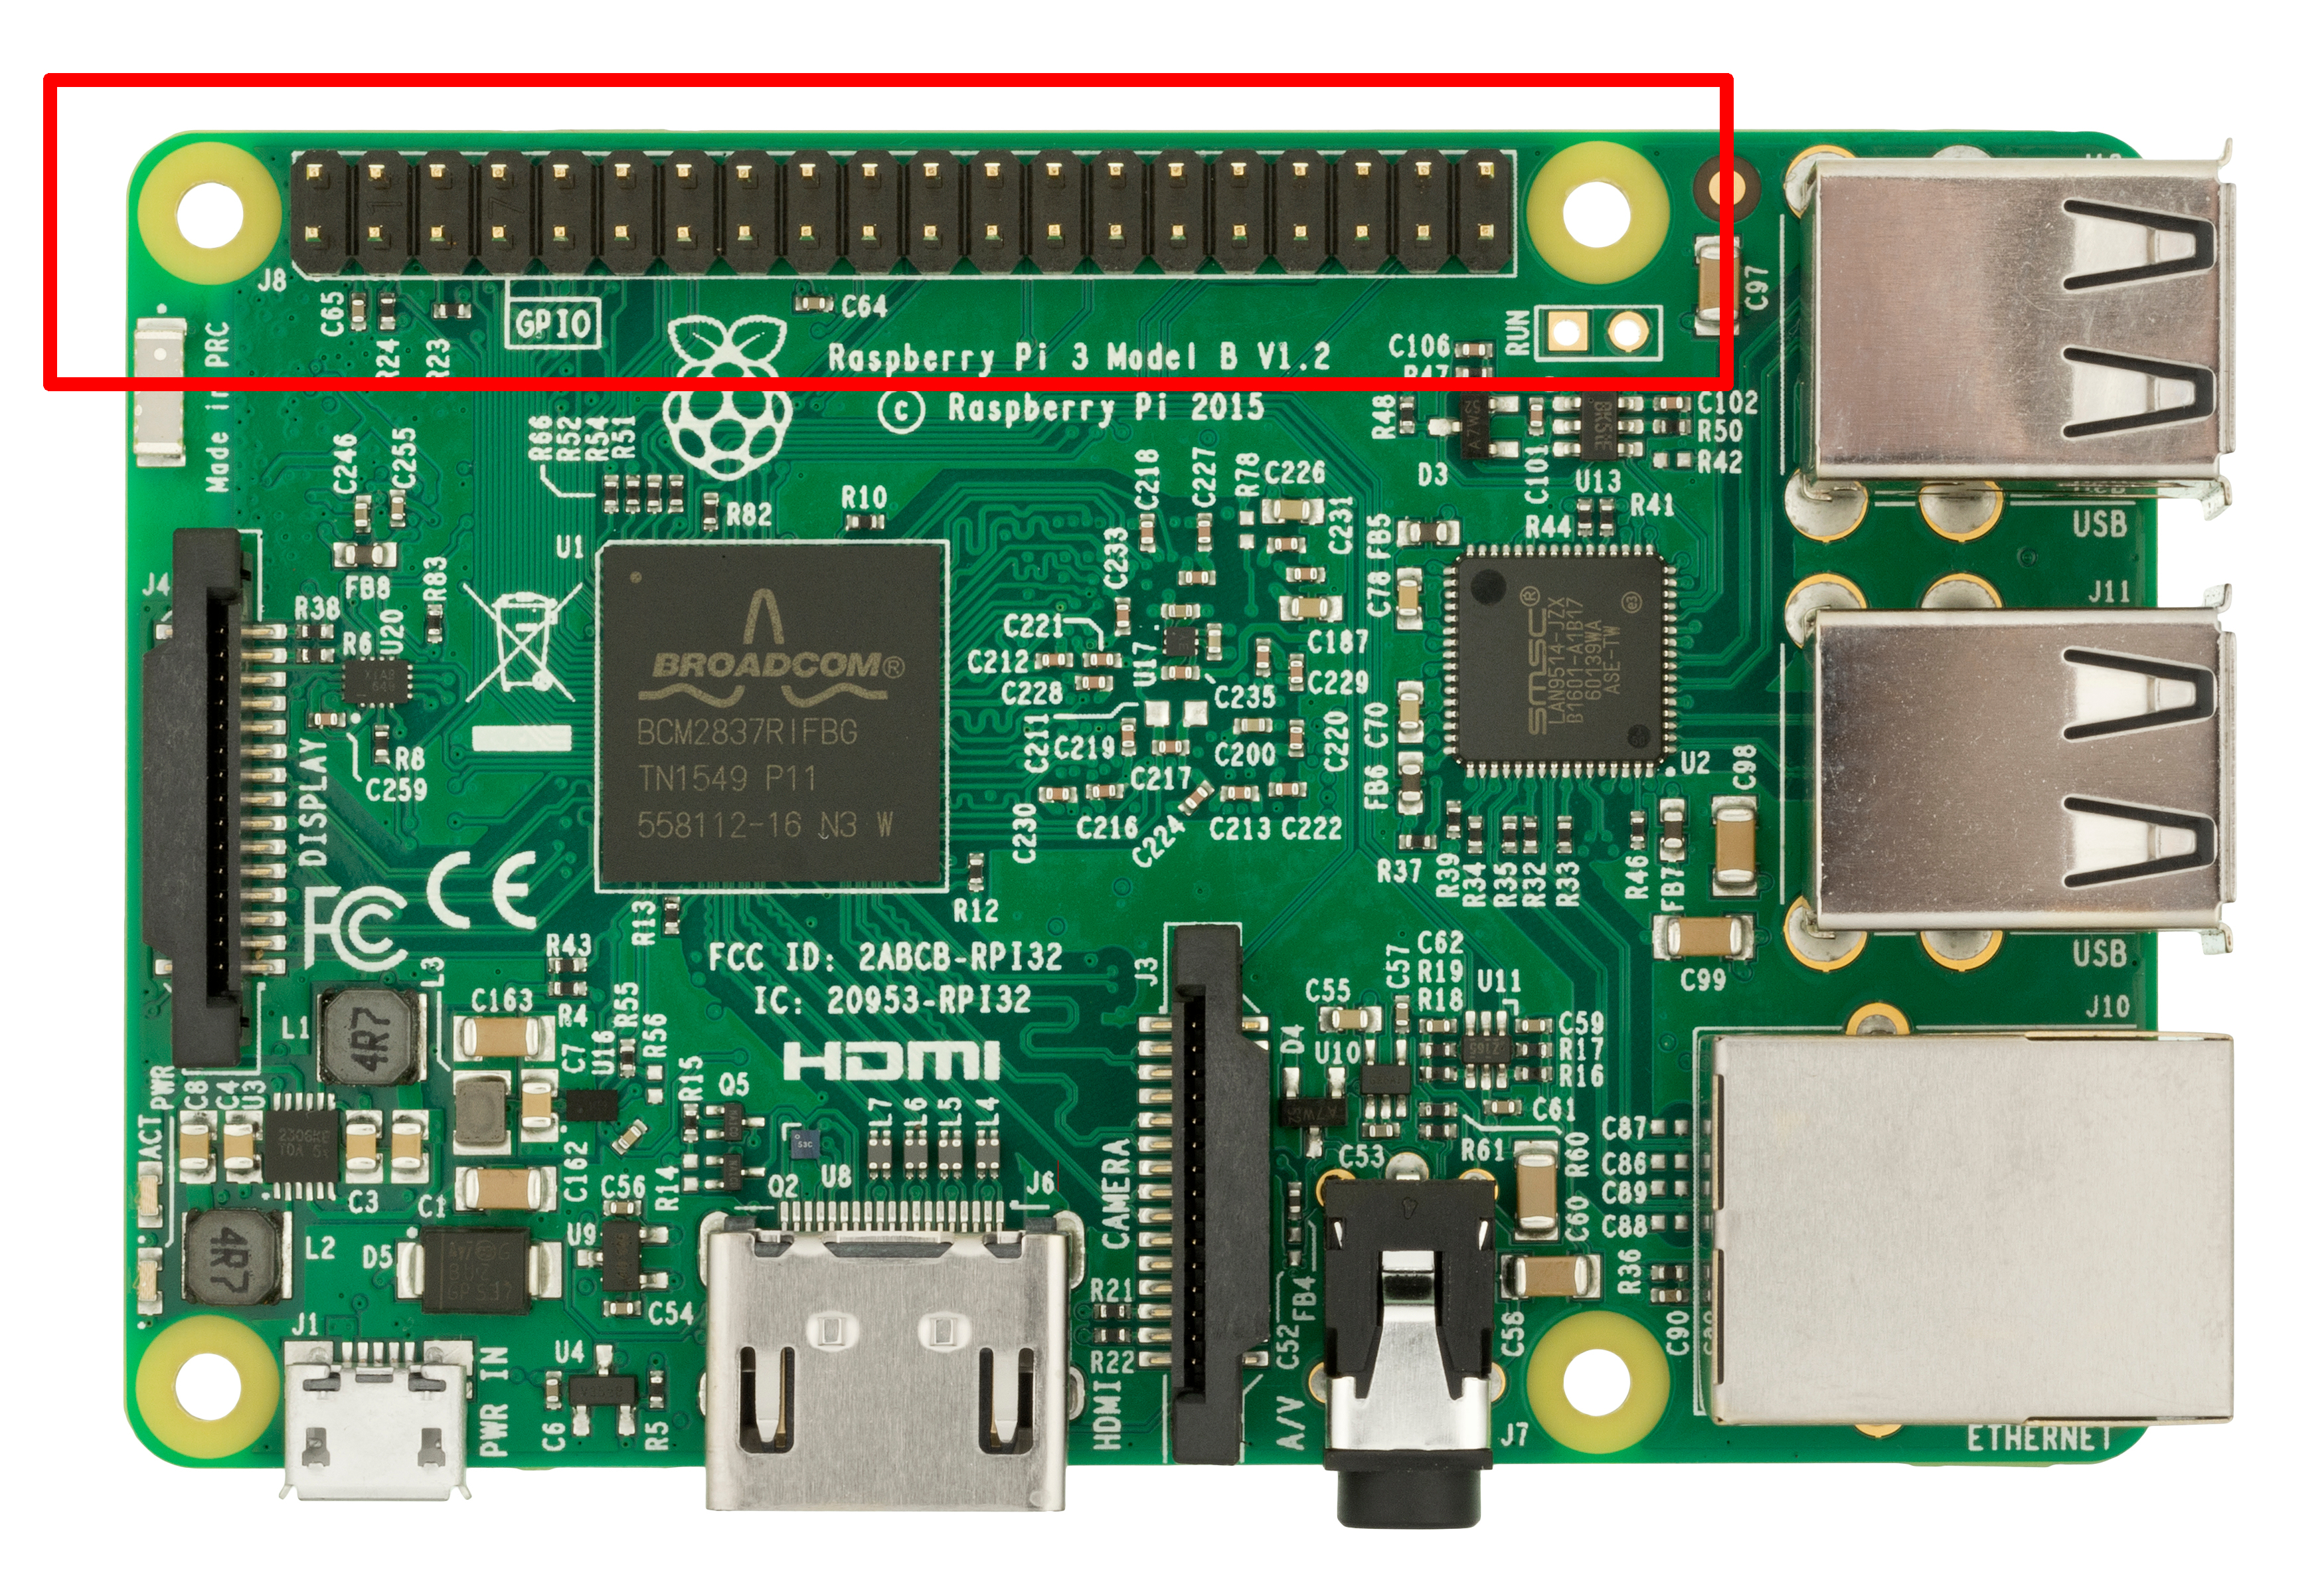
\includegraphics[scale=0.30]{\imageDir/rpi-border-gpio.jpg}
	\caption{Raspberry-Pi 3}
	\label{fig:rpi-border-gpio}
\end{figure}

Die Pin-Belegung\footnote{\url{http://www.netzmafia.de/skripten/hardware/RasPi/Projekt-PIR/}} des HC-SR501

\begin{figure}[h]
	\centering
	\includegraphics[scale=0.60]{\imageDir/PIR4.jpg}
	\caption{Pin-Schema HC-SR501}
	\label{fig:PIR4}
\end{figure}

ist wie folgt definiert:
\begin{itemize}
	\item Pin 1: VCC (5 Volt)
	\item Pin 2: Out, Data
	\item Pin 3: GND, Masse
\end{itemize}
\ \newpage
Zusätzlich kann die Empfindlichkeit und Haltezeit an den beiden Drehreglern eingestellt werden. Zusätzlich kann noch das Daten-Pin Verhalten über den Jumper konfiguriert werden.

\subsection{GPIO}
\emph{GPIO} ist die Abkürzung für \emph{General Purpose Input/Output}. Man bezeichnet damit programmierbare Ein- und Ausgänge für allgemeine Zwecke. Die \emph{GPIOs} werden als Lötpunkt oder Pin in Form einer Stiftleiste herausgeführt und dienen als Schnittstelle zu anderen Systemen oder Schaltungen, um diese über den \emph{Raspberry Pi} zu steuern. Dabei kann der \emph{Raspberry Pi} bei entsprechender Programmierung digitale Signale von außen annehmen \emph{(Input)} oder Signale nach außen abgeben \emph{(Output)}.
\newline
\newline
Viele der \emph{GPIOs} erfüllen je nach Einstellung und Programmierung verschiedene Funktionen. Neben den typischen \emph{GPIO}-Ein- und Ausgängen finden sich aber auch Pins mit der Doppelfunktion für \emph{I2C, SPI} und eine serielle Schnittstelle.

\subsubsection{HC-SR501 GPIO Verbindung}
Für den HC-SR501 wird die Pin-Belegung wie folgt gewählt:

\begin{itemize}
	\item Pin 1: VCC (5 Volt) an Pin 2
	\item Pin 2: Out, Data an Pin 8
	\item Pin 3: GND an Pin 6
\end{itemize}
\ \newline
Diese Pin-Belegung erfolgt aufgrund der folgenden schematischen Darstellung\footnote{\url{http://pi4j.com/pins/model-3b-rev1.html}}:

\begin{figure}[h]
	\centering
	\includegraphics[scale=1.30]{\imageDir/j8header-3b.png}
	\caption{Pin-Schema}
	\label{fig:j8header-3b}
\end{figure}
\newpage

\subsection{Betriebssysteme}
Dieser Abschnitt behandelt die verwendete Betriebssysteme für den \emph{Raspberry PI}. Die Applikation \emph{RPISec} wurde einerseits mit dem Betriebssystem \emph{HypriotOS} und andererseits mit \emph{Raspian} realisiert. Das Betriebssystem \emph{HypriotOS} basiert auf \emph{Debian Jessie} und wird von dem \emph{OpenSource} Projekt \emph{Hypriot}\footnote{\url{https://blog.hypriot.com/}} zur Verfügung gestellt. Das Ziel von \emph{HypriotOS} ist es ein Betriebssystem für den \emph{Raspberry PI} zur Verfügung stellen, das bereits Docker vorinstalliert und betriebsbereit hat. Mit dem Betriebssystem \emph{Raspian} muss Docker selbst installiert werden, wobei Docker als Paket im \emph{Repository} zur Verfügung steht und daher sich die Installation als unkompliziert gestaltet.
\newline
\newline
Wenn Docker installiert und betriebsbereit ist, dann spielt es keine Rolle auf welchem Betriebssystem die Applikation \emph{RPISec} betrieben wird, solange dieses Betriebssystem auf einer von \emph{Docker} unterstützten Kernelversion aufbaut.
\newline
\newline
Da die Applikation \emph{RPISec} auf eine aktive Internetverbindung angewiesen ist, muss das Betriebssystem so konfiguriert werden, dass der \emph{Raspberry PI} entweder über \emph{Ethernet} oder \emph{Wlan} an ein Netzwerk angebunden ist, das Zugriff auf das Internet erlaubt. In einem produktiven Betrieb muss der \emph{Raspberry PI} über das Internet erreichbar sein, damit die mobilen \emph{Clients} Anfragen an die gehosteten \emph{Microservice} absetzen können.
\begin{figure}[h]
	\centering
	\includegraphics[scale=0.5]{\imageDir/hypriot-logo.jpg}
	\caption{HypriotOS}
	\label{fig:HypriotOS}
\end{figure}\begin{figure}[h]
	\centering
	\includegraphics[scale=0.15]{\imageDir/raspbian-logo.png}
	\caption{RaspianOS}
	\label{fig:RaspianOS}
\end{figure}

\section{Software und Dienste}
Dieser Abschnitt behandelt die verwendete bzw. implementierte Software und die verwendeten Dienste für die Applikation \emph{RPISec}.

\subsection{\emph{Microservices}}
Dieser Abschnitt behandelt die auf dem \emph{Raspberry PI} gehosteten Services. Die Services wurden mit \emph{Spring Boot} als \emph{Microservices} implementiert, was möglich war, da Oracle eine ARM Implementierung der Java-JDK bereitstellt und die \emph{Microservices} schlank implementiert wurden, sodass die zur Verfügung stehenden Ressourcen ausreichen, um diese Services auf einen \emph{Raspberry PI} zu betreiben.
\newline
\newline
Es wurden die beiden \emph{Microservices Auth-Service} für die Benutzerverwaltung und OAuth2 Authentifizierung und \emph{App-Service} für die Interaktion mit der Sensorapplikation und der Interaktion mit dem \emph{Cloud} Dienst implementiert, wobei der \emph{Microservice Auth-service} im Zuge des Projekts für die Lehrveranstaltung \emph{Service Engineering} implementiert wurde. Es hätte auch ausgereicht die Benutzerverwaltung in den \emph{Microservice App-Service} zu verpacken, obwohl dann der \emph{Microservice} für zwei Aspekte verantwortlich gewesen wäre, was im Widerspruch zu einem \emph{Microservice} steht, der nur für einen Aspekt verantwortlich sein soll. 
\newline
\newline
Der \emph{Microservice App-Service} interagiert nicht direkt mit der Sensorik, sondern bindet die Sensorapplikation beschrieben in Abschnitt \ref{sec:sensor-application} ein und ist für dessen Lebenszyklus verantwortlich. Nachdem Start der Sensorapplikation wird ein \emph{Listener} registriert, der auf Statusänderungen des Bewegungssensor reagiert und diesen Sicherheitsverstoß wie in Abbildung \ref{fig:image-sequence-incident} behandelt.

\subsection{Datenbank}
Dieser Abschnitt behandelt die verwendete Datenbank für die \emph{Microservices}. Im Entwicklungsbetrieb auf einen Entwicklerrechner wird die Datenbank H2 und im produktiven Betrieb auf einen \emph{Raspberry PI} die Datenbank PostgreSQL verwendet. Die Datenbank PostgreSQL konnte am \emph{Raspberry PI} verwendet werden, da PostgreSQL die ARM Architektur unterstützt und sich auch mit geringen Ressourcenaufwand betreiben lässt.

\subsection{\emph{Cloud} Dienst}
Dieser Abschnitt behandelt den verwendeten \emph{Cloud} Dienst \emph{Firebase}. \emph{Firebase} ist ein \emph{Cloud} Dienst von \emph{Google}, der einen \emph{Messaging} Dienst sowie eine Onlinedatenbank (JSON-Datenbank) bereitstellt. Bis zu einer gewissen Anzahl von \emph{Requests} ist dieser Dienst kostenlos zu verwenden.  
\newline
\newline
Für \emph{Firebase} gibt es eine Java Implementierung das sogenannte \emph{firebase-admin-sdk}, das eine API zum Interagieren mit der JSON-Datenbank und eine API zum Erstellen von Authentifizierungstoken für die \emph{Client}-Authentifizierung auf \emph{Firebase} zur Verfügung stellt. In der Java Implementierung wird zurzeit keine API für die Interaktion mit dem \emph{Messaging} Dienst zur Verfügung gestellt, was aber kein Problem darstellt, da es sich hierbei um eine einfache Anfrage an eine \emph{REST-API} handelt, die mit Spring \emph{RestTemplate} realisiert wurde.
\newline
\newline
Für die Interaktion mit \emph{Firebase} über \emph{Android} wird ebenfalls eine Java Implementierung bereitgestellt. Diese Implementierung enthält auch eine \emph{API} für den \emph{MEssaging} Dienst von \emph{Firebase}.
\newline
\newline
Es sind zwar Implementierungen der \emph{API} mehrere Programmiersprachen verfügbar, jedoch wird eine vollständige \emph{API} nur für \emph{NodeJS} bereitgestellt.

\subsection{\emph{Docker}}
Dieser Abschnitt behandelt die Verwendung von \emph{Docker}, für das hosten der Services und Datenbanken für die Services. Dank dem \emph{Raspberry PI Image}, bereitgestellt von \emph{Hypriots}, sind bereits \emph{Docker} und \emph{Docker-Compose} \emph{(Orchestration)} vorinstalliert und müssen nicht separat geladen und für die Zielarchitektur gebaut werden.
\newline
\newline
Da der Umgang mit \emph{Docker} und einer umfangreicheren Infrastruktur mit viel Shell-Skripten verbunden ist, wird das Python basierte Tool \emph{Docker-Compose} verwendet, das es erlaubt eine Infrastruktur, die aus einer Menge von untereinander abhängigen Services besteht, deklarativ über eine \emph{YAML}-Konfigurationsdatei zu konfigurieren und zu \emph{orchestrieren}. 
\newline
\newline
Die Definition der \emph{Images} sowie der Aufbau der \emph{Docker-Compose} Infrastruktur sind im Verzeichnis \emph{$/host/docker/$} enthalten, wobei die einzelnen \emph{Dockerfiles} der Services in Unterverzeichnissen organisiert werden, die alle Abhängigkeiten, welche in die Images mitaufgenommen werden müssen, enthalten. Die \emph{PostgreSQL} Images stehen am \emph{Docker Hub}\footnote{https://hub.docker.com/r/tobi312/rpi-postgresql/} zur Verfügung. Es wurde ein eigenes Basisimage definiert, das die benötigten Abhängigkeiten für die Interaktion mit der Hardware beinhaltet. Es werden in diesem Basisimage alle benötigten C-Bibliotheken wie \emph{WiringPI}\footnote{https://git.drogon.net/?p=wiringPi;a=summary} und die Bibliotheken für das Interagieren mit der \emph{Raspberry Pi GPU}\footnote{https://github.com/raspberrypi/userland} während des Bauens des Images geladen und kompiliert. Dieser Ansatz wurde gewählt, da das Bauen der Abhängigkeiten aufwendig ist und viel Zeit in Anspruch nimmt und sich dieses Basisimage nur selten ändert.
\begin{center}
	\begin{figure}[h]
		\centering
		\includegraphics[scale=0.65]{\imageDir/pi-docker-infrastructure.jpg}
		\caption{\emph{Raspberry PI Docker} Infrastruktur}
		\label{fig:rapsi-docker-infrastructure}
	\end{figure}
\end{center}
Die Abbildung \ref{fig:rapsi-docker-infrastructure} zeigt die implementierte \emph{Docker} Infrastruktur, wie sie am \emph{Raspberry PI} gehostet wird. Da die Daten der \emph{Docker-Container} persistent gehalten werden müssen, werden die Daten in den \emph{Containern} in Verzeichnissen gehalten, die auf den \emph{Host} über ein \emph{Volume Mapping} gebunden sind. Der \emph{Docker Container App-Service} benötigt privilegierte Rechte, damit die Sensorapplikation mit der angeschlossenen \emph{Hardware} des \emph{Raspberry PI} kommunizieren kann. 
\newline
\newline
Der Quelltext \ref{src:test-docker-compose} zeigt den Inhalt der \emph{docker-compose.yml}, welche die \emph{Docker} Infrastruktur für \emph{RPISec} am \emph{Raspberry PI} definiert. Die in der Datei vorkommenden Textfragmente im Format \emph{\$\{...\}} stellen Variablen dar, die \emph{Docker-Compose} entweder aus einer Datei mit dem Namen \emph{.env}, die auf derselben Ebene wie die \emph{docker-compose.yml} platziert werden muss, oder aus den Umgebungsvariablen des Benutzers, mit dem die Infrastruktur erstellt wird, auflöst. Sollten Variablen nicht auflösbar sein, so wird eine entsprechende Meldung auf die Konsole ausgegeben.
\begin{code}
	\caption{docker-compose.yml für RPISec am \emph{Raspberry PI}}
	\yamlFile{\dockerRPIDir/docker-compose.yml}
	\label{src:test-docker-compose}
\end{code}
\ \newline
Das Bauen der Infrastruktur und Starten der Services dauert am \emph{Raspberry PI} relativ lange, da nur wenig Speicher zur Verfügung steht, es sich um eine ARM-Architektur handelt und das Speichermedium eine \emph{MicroSD} Karte ist. Ebenso ist die Performance der Services nicht herausragend, jedoch kann die Applikation auf dem \emph{Raspberry PI} problemlos ausgeführt werden.  
\subsection{Sensor Applikation}

Bei den Komponenten der Sensor-Anwendung handelt es sich, wie in \autoref{sec:raspberrypi} erwähnt, um die beiden Bauteile:

\begin{itemize}
	\item \emph{AZDeliveryCamRasp Kamera}
	\item \emph{HC-SR501 Bewegungssensor}
\end{itemize}

\subsection{Kamera}

Bei der Kamera handelt es sich um ein eigens für den Raspberry Pi entwickeltes Modell und wird direkt an den vorhanden Kamera-Port des Raspberry Pi 3\footnote{\url{https://en.wikipedia.org/wiki/Raspberry_Pi\#/media/File:Raspberry-Pi-3-Flat-Top.jpg}} angeschlossen.

\begin{figure}[h]
	\centering
	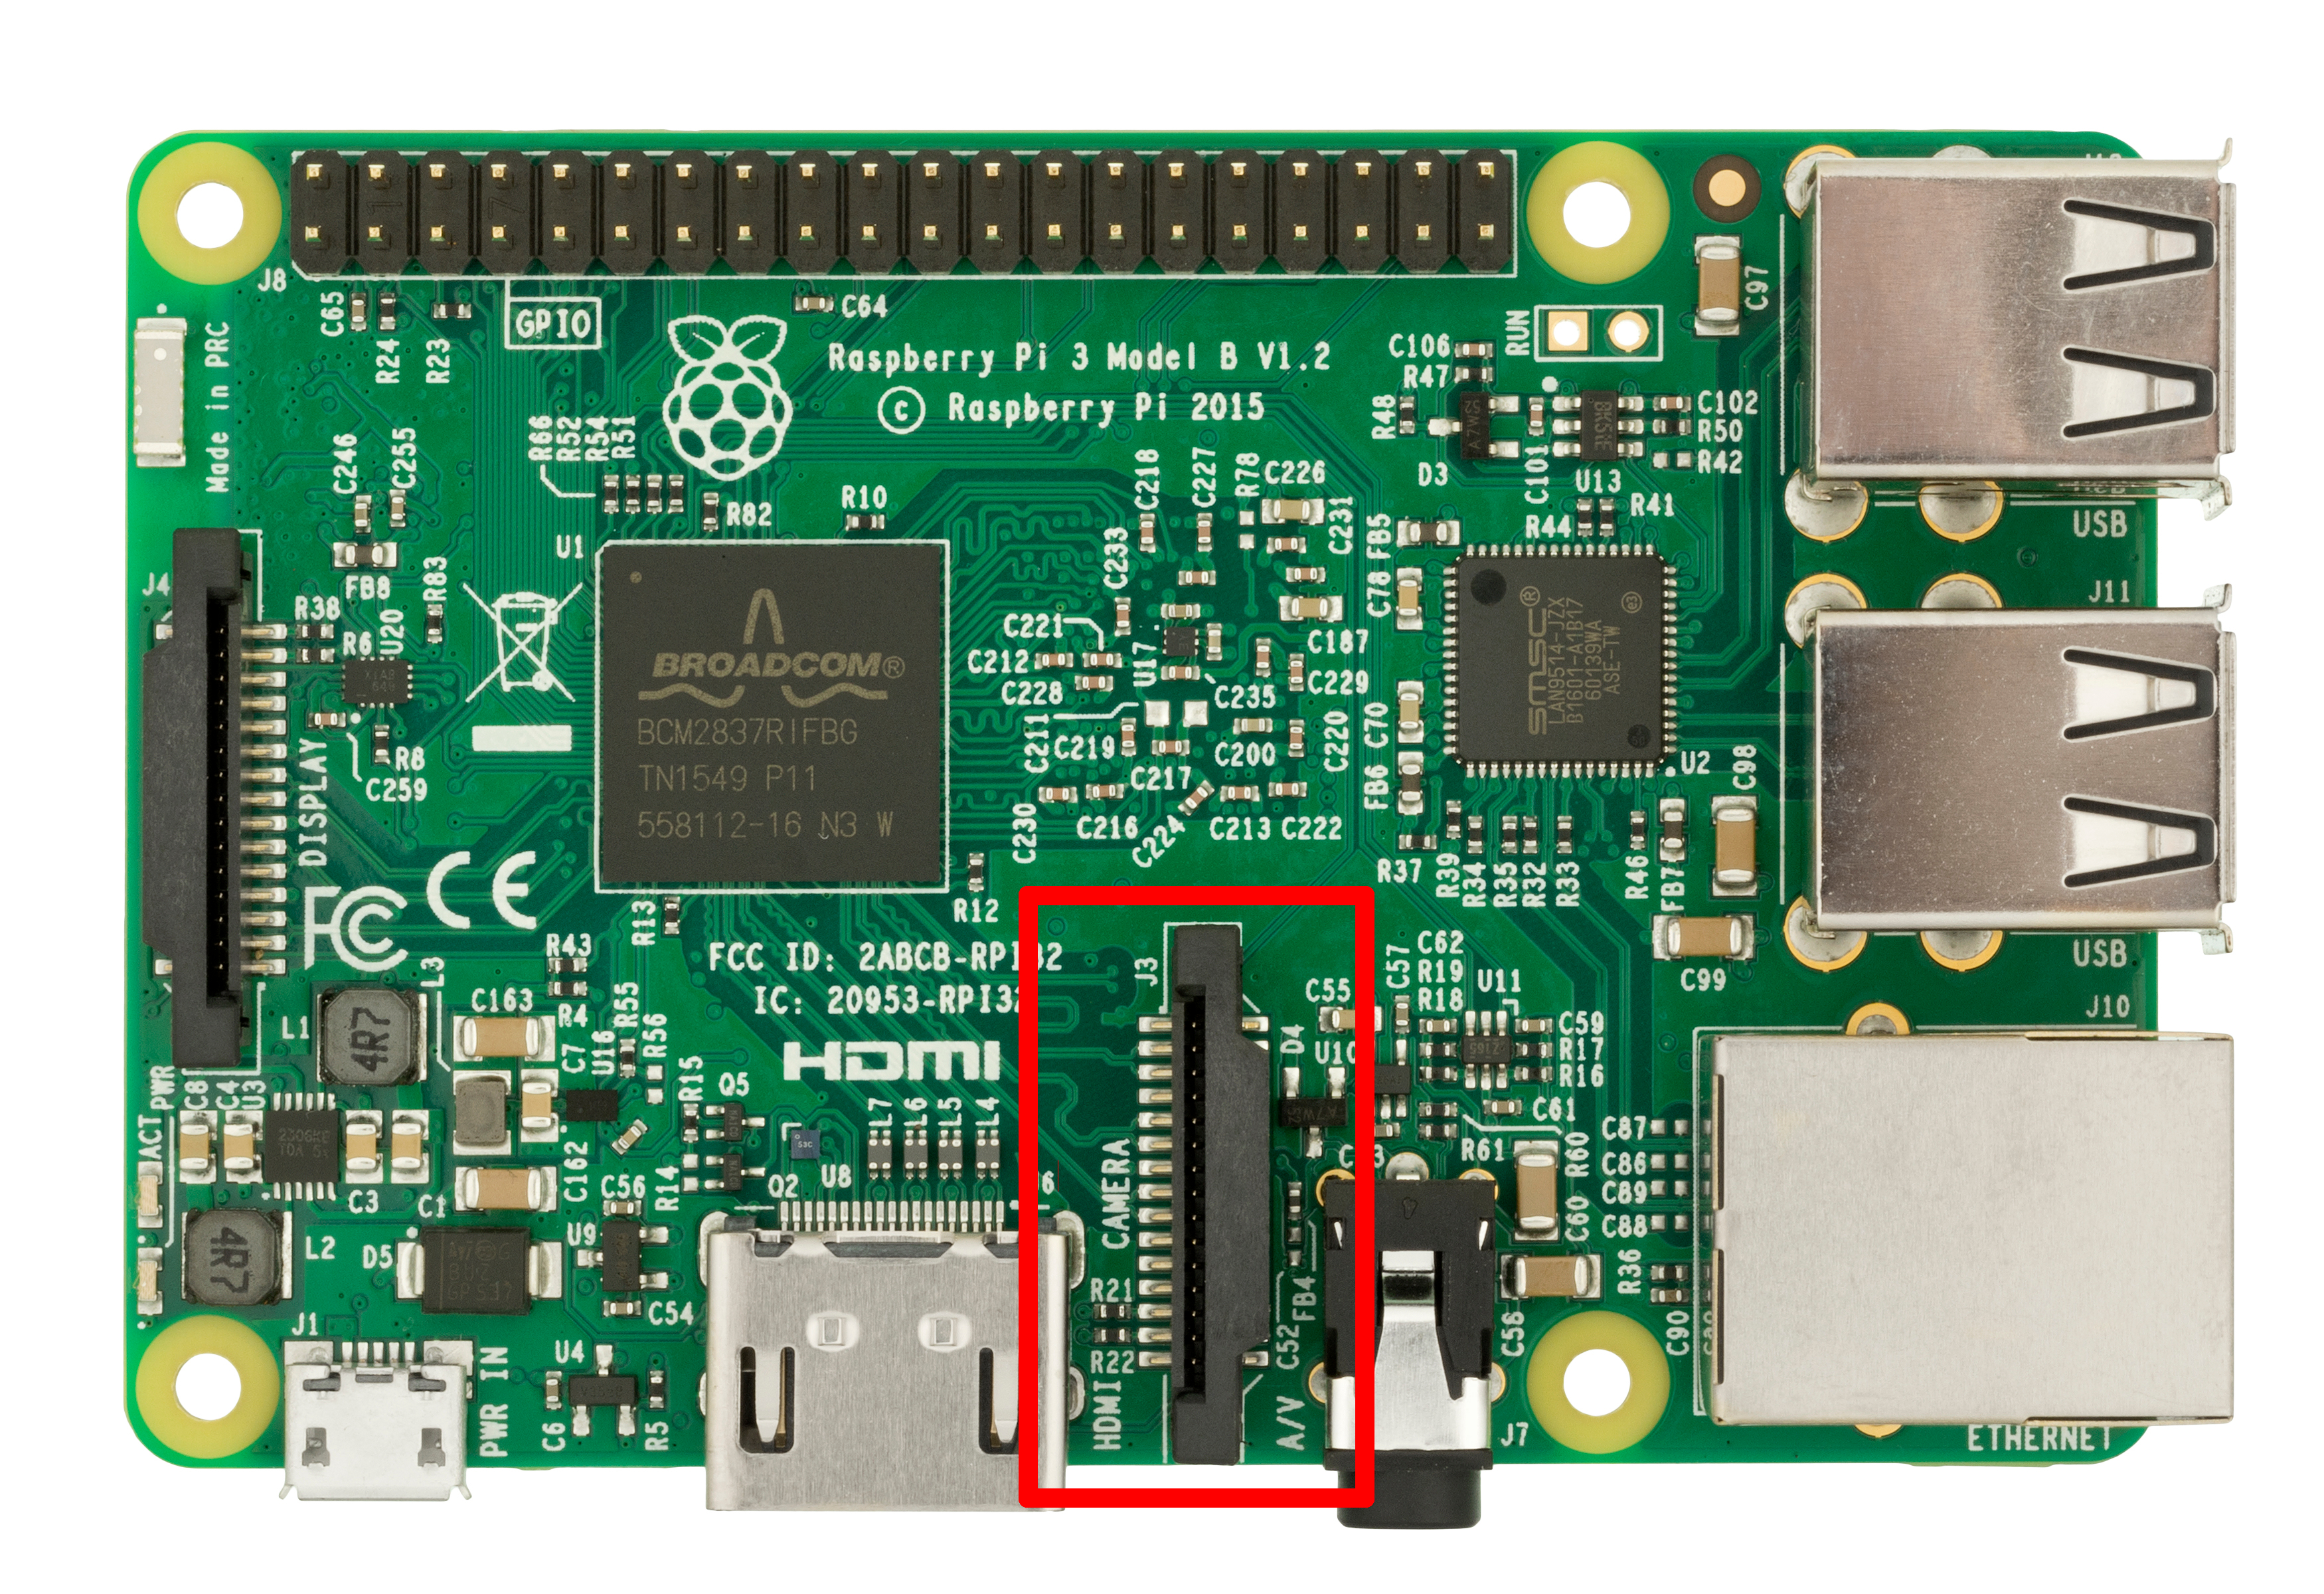
\includegraphics[scale=0.20]{\imageDir/rpi-border-cam.jpg}
	\caption{Raspberry-Pi 3}
	\label{fig:rpi-border-cam}
\end{figure}

Anschließend muss die Kamera aktiviert werden. Dies geschieht über das, mit den meisten Linux-Distributionen mitgelieferte, Programm \emph{raspi-config\footnote{\url{https://upload.wikimedia.org/wikipedia/commons/e/ed/Raspi-config.png}}}. Dieses Programm wird auch benutzt um andere Komponenten des Raspberry Pi zu konfigurieren.

\begin{figure}[h]
	\centering
	\includegraphics[scale=0.40]{\imageDir/raspi-config-cam.png}
	%By Onepiece84 (Own work) [CC BY-SA 4.0 (http://creativecommons.org/licenses/by-sa/4.0)], via Wikimedia Commons
	\caption{Raspi-config}
	\label{fig:raspi-config-cam}
\end{figure}

Zur Ansteuerung der Kamera wird das Konsolenprogramm \emph{raspistill} verwendet. Diese kann mit verschiedensten Parametern konfiguriert werden. Als Beispiel:\\
\newline
\begin{code}
	raspistill --width 1920 --height 1080 -o test.jpg\\
\end{code}
\newline
Dies erzeugt ein Bild in der Auflösung 1920 x 1080 Pixel und speichert es unter dem Dateinamen \emph{test.jpg}.

\subsection{HC-SR501 Bewegungssensor}

Der HC-SR501 Sensor wird über die GPIO-Pins des Raspberry Pi angesteuert. Hierbei werden Masse, Stromversorgung und Daten-Pin des HC-SR501 Sensors mit den GPIO-Pins verbunden. 

\begin{figure}[h]
	\centering
	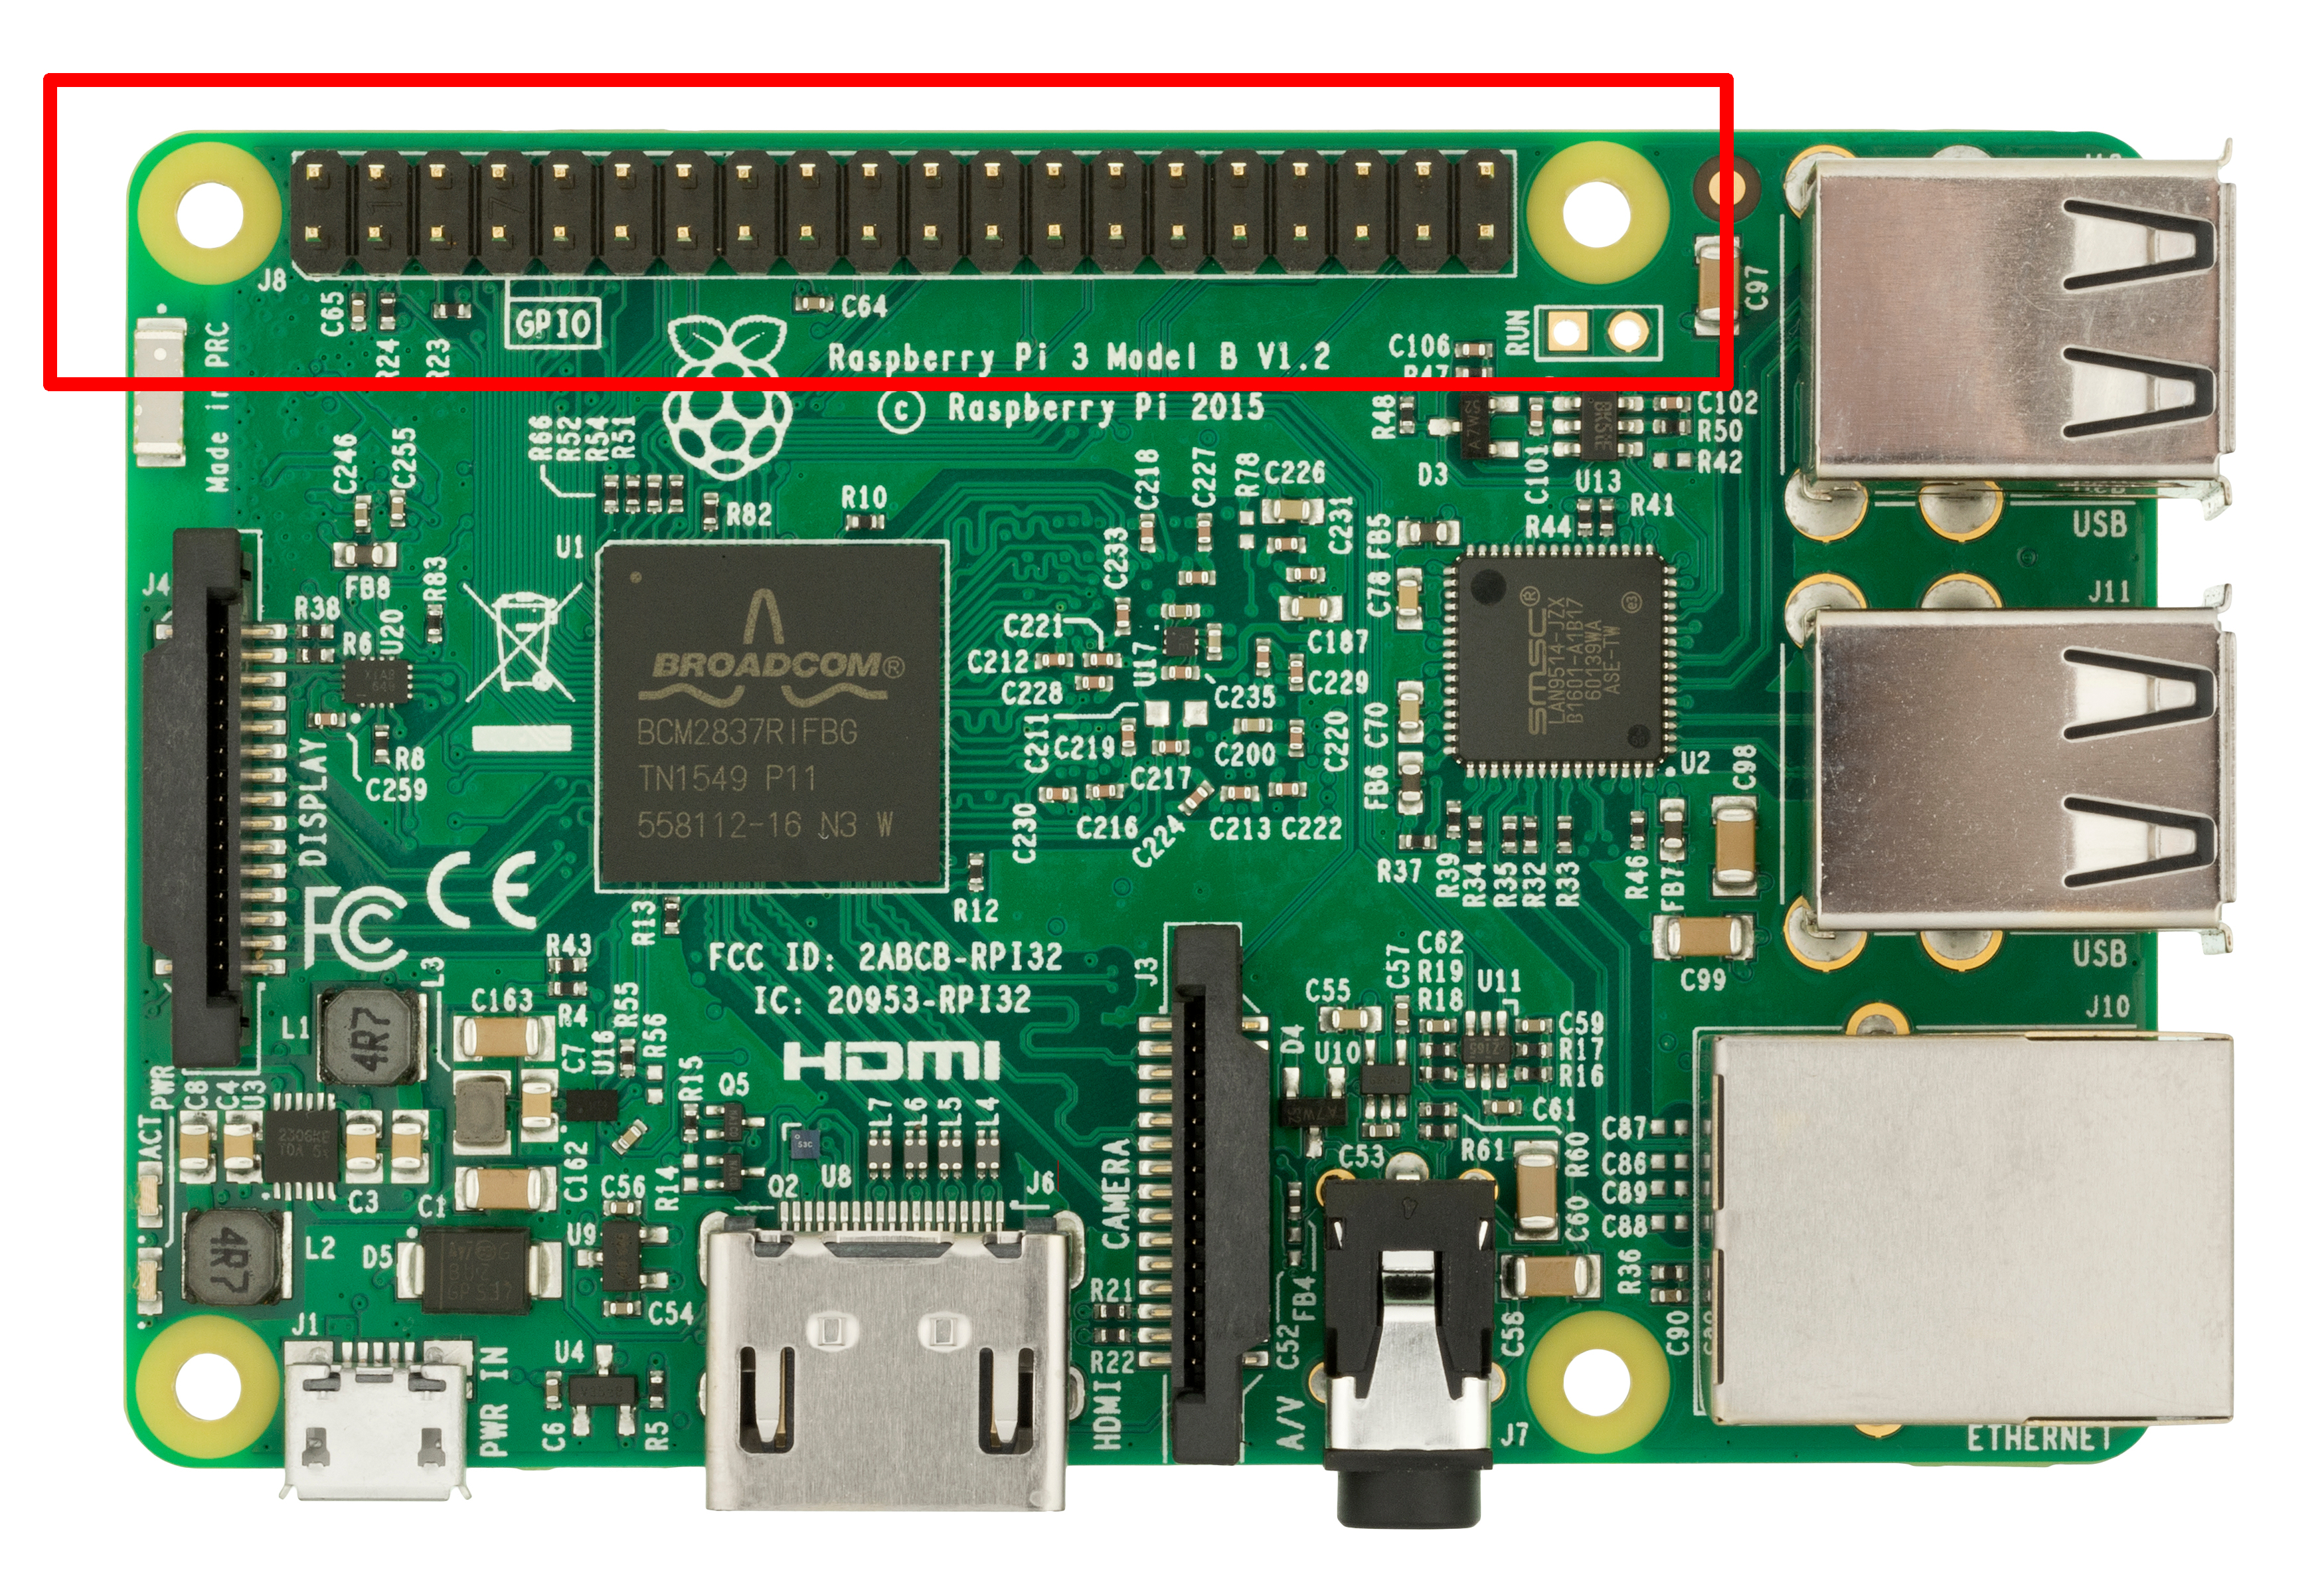
\includegraphics[scale=0.20]{\imageDir/rpi-border-gpio.jpg}
	\caption{Raspberry-Pi 3}
	\label{fig:rpi-border-gpio}
\end{figure}

Die Pin-Belegung\footnote{\url{http://www.netzmafia.de/skripten/hardware/RasPi/Projekt-PIR/}} des HC-SR501

\begin{figure}[h]
	\centering
	\includegraphics[scale=0.50]{\imageDir/PIR4.jpg}
	\caption{Pin-Schema HC-SR501}
	\label{fig:PIR4}
\end{figure}

ist wie folgt definiert:

\begin{itemize}
	\item Pin 1: VCC (5 Volt)
	\item Pin 2: Out, Data
	\item Pin 3: GND, Masse
\end{itemize}

zusätzlich kann die Empfindlichkeit und Haltezeit an den beiden Drehreglern eingestellt werden. Zusätzlich kann noch das Daten-Pin Verhalten über den Jumper konfiguriert werden.

\pagebreak

\subsection{GPIO}

GPIO ist die Abkürzung für General Purpose Input Output. Man bezeichnet damit programmierbare Ein- und Ausgänge für allgemeine Zwecke. Die GPIOs werden als Lötpunkt oder Pin in Form einer Stiftleiste herausgeführt und dienen als Schnittstelle zu anderen Systemen oder Schaltungen, um diese über den Raspberry Pi zu steuern. Dabei kann der Raspberry Pi bei entsprechender Programmierung digitale Signale von außen annehmen (Input) oder Signale nach außen abgeben (Output).\\

Viele der GPIOs erfüllen je nach Einstellung und Programmierung verschiedene Funktionen. Neben den typischen GPIO-Ein- und Ausgängen finden sich aber auch Pins mit der Doppelfunktion für I2C, SPI und eine serielle Schnittstelle.\\

\subsubsection{HC-SR501 GPIO Verbindung}

Für den HC-SR501 wird die Pin-Belegung wie folgt gewählt:

\begin{itemize}
	\item Pin 1: VCC (5 Volt) an Pin 2
	\item Pin 2: Out, Data an Pin 8
	\item Pin 3: GND an Pin 6
\end{itemize}

Diese Pin-Belegung erfolgt aufgrund der folgenden schematischen Darstelleung\footnote{\url{http://pi4j.com/pins/model-3b-rev1.html}}:

\begin{figure}[h]
	\centering
	\includegraphics[scale=1.00]{\imageDir/j8header-3b.png}
	\caption{Pin-Schema}
	\label{fig:j8header-3b}
\end{figure}

\pagebreak

\subsection{Pin-Ansteuerung mit Java}

Die Ansteuerung der Pins erfolgt über die \emph{Pi4J\footnote{\url{http://pi4j.com/}}}-Bibliotheken die wiederum die \emph{WiringPi\footnote{\url{http://wiringpi.com/}}}-Bibliothek nutzt, welche die eigentliche Ansteuerung der Pins erledigt.

\subsubsection{Pi4J}
Pi4J ist eine Bibliothek  für Java, die den vollen Zugriff auf die Ressourcen des Raspberry PI ermöglicht. Mit Pi4J ist es möglich Anwendungen für Raspberry PI zu schreiben, die nur Java benötigen. Damit können praktisch alle Bibliotheken eingesetzt werden, die für Java verfügbar sind. Einschränkungen gibt es nur bei den Ressourcen des Raspberry.

\subsubsection{WiringPi}
WiringPi ist ein nützliches Framework um die GPIO Ein-und Ausgänge am Raspberry Pi zu schalten. Das Ziel dieser Bibliothek ist es, eine einzige gemeinsame Plattform und Programmierschnistelle für den Zugriff auf die GPIOs des Rapsberry Pi für verschiedene Programmiersprachen zur Verfügung zu stellen. Im Kern ist WiringPi eine C-Bibliothek, aber sie steht auch in Ruby und Python zur Verfügung.

\begin{code}
	\caption{gpio-controller.java}
	\yamlFile{\srcDir/gpio-controller.java}
	\label{src:gpio-controller}
\end{code}
\subsection{Mobiler \emph{Client}}

Beim RPISEC-Client handelt es sich um eine native Android App. Diese kommuniziert über REST-Schnittstellen mit einem OAuth-Server sowie mit Firebase-Diensten von Google. Die für diese App verwendeten Firebase-Dienste sind Firebase-Messaging und Firebase-RealTimeDatabase.\\

\subsubsection{Login}

Die Startseite der App besteht nur aus einem Login-Fenster (\autoref{fig:android_login}). Der Login erfolgt in zwei Schritten.

\begin{enumerate}
	\item OAuth Login\\
	\newline
	Die App generiert einen UUID-Wert (Universally Unique Identifier) als Identifikator für das Gerät. Zusammen mit dem eingegebenen Benutzernamen, Passwort und der UUID wird eine Anfrage für einen OAuth-Token an den OAuth-Server gestellt. Sind die Zugangsdaten korrekt, wird für diese UUID ein Token, sowie Client-Id und Client-Secret erzeugt und als Antwort an die App übertragen. Der OAuth-Token wird für die Authentifizierung bei den verbunden Diensten benutzt.\\
	
	\begin{code}
		\caption{ClientLoginOAuthTask.java}
		\javaFile{\srcDir/ClientLoginOAuthTask.java}
		\label{src:ClientLoginOAuthTask}
	\end{code}
	
	\pagebreak
	
	\item  Firebase Login\\
	\newline
	Im zweiten Schritt wird ein Token für Firebase-Messaging registriert. Dies erfolgt wiederum mit dem Benutzernamen und Passwort. Nach der Registrierung kann die App Nachrichten über den Firebase-Messageing Dienst empfangen.\\
	
	\begin{code}
		\caption{RegisterFCMTask.java}
		\javaFile{\srcDir/RegisterFCMTask.java}
		\label{src:RegisterFCMTask}
	\end{code}
\end{enumerate}

\begin{figure}[h]
	\centering
	\includegraphics[scale=0.5]{\imageDir/android_login.png}
	\caption{Pin-Schema}
	\label{fig:android_login}
\end{figure}

Nach einem erfolgreichen Login wird automatisch die Detailansicht (siehe \autoref{fig:android_image_overview_m}) gestartet.

\pagebreak

\subsubsection{Detailansicht}

Bei der Detailansicht handelt es sich um eine Übersicht aller Bilder, chronologisch geordnet nach Aufnahmedatum, in einem Raster. Bei den angezeigten Bildern handelt es sich nur um Thumbnails. Die richtigen Bilder werden beim Auswählen eines Bildes angezeigt, ähnlich dem Fotoviewer in Android.\\

Die Detailansicht wird beim Eintreffen eines neuen Bildes aktualisiert. Sollte die Detailansicht nicht die aktive Anwendung sein, wird in der Infoleiste eine Notifikation angezeigt und ein Ton abgespielt. Durch tippen auf die Notifikation wird die Anwendung wieder in den Vordergrund geholt.\\

Mittels Swipe-Down-Geste kann die Ansicht aktualisiert werden.

\begin{figure}[h]
	\centering
	\includegraphics[scale=0.7]{\imageDir/android_image_overview_m.png}
	\caption{Pin-Schema}
	\label{fig:android_image_overview_m}
\end{figure}

\subsubsection{Datenabfrage}

Bei jedem \emph{Incident} der von der Server-Anwendung über Firebase-Messaging an die App gesendet wird, werden der Titel, eine Nachricht und die Id des aufgenommenen Bildes übertragen. Mit dieser Id kann das eigentliche Bild aus der Firebase-RealTimeDatabase abgerufen werden.\\

\begin{code}
	\caption{FirebaseMessaging.java}
	\javaFile{\srcDir/FirebaseMessaging.java}
	\label{src:FirebaseMessaging}
\end{code}
\subsection{\emph{Docker}}
Dieser Abschnitt behandelt die Verwendung von \emph{Docker}, für das hosten der Services und Datenbanken für die Services. Dank dem \emph{Raspberry PI Image}, bereitgestellt von \emph{Hypriots}, sind bereits \emph{Docker} und \emph{Docker-Compose} \emph{(Orchestration)} vorinstalliert und müssen nicht separat geladen und für die Zielarchitektur gebaut werden.
\newline
\newline
Da der Umgang mit \emph{Docker} und einer umfangreicheren Infrastruktur mit viel Shell-Skripten verbunden ist, wird das Python basierte Tool \emph{Docker-Compose} verwendet, das es erlaubt eine Infrastruktur, die aus einer Menge von untereinander abhängigen Services besteht, deklarativ über eine \emph{YAML}-Konfigurationsdatei zu konfigurieren und zu \emph{orchestrieren}. 
\newline
\newline
Die Definition der \emph{Images} in Form von \emph{Dockerfiles} sowie der Aufbau der \emph{Docker-Compose} Infrastruktur sind im Verzeichnis \emph{$/host/docker/$} enthalten, wobei die einzelnen \emph{Dockerfiles} der Services in Unterverzeichnissen organisiert wurden, die alle Abhängigkeiten, welche in die Images mitaufgenommen werden müssen, enthalten. Die \emph{PostgreSQL} Images stehen am \emph{Docker Hub}\footnote{https://hub.docker.com/r/tobi312/rpi-postgresql/} zur Verfügung. Es wurde ein eigenes Basisimage definiert, das die benötigten Abhängigkeiten für die Interaktion mit der Hardware beinhaltet. Es werden in diesem Basisimage alle benötigten C-Bibliotheken wie \emph{WiringPI}\footnote{https://git.drogon.net/?p=wiringPi;a=summary} und die Bibliotheken für das Interagieren mit der \emph{Raspberry Pi GPU}\footnote{https://github.com/raspberrypi/userland} während des Bauens des Images geladen und für die Zielplattform kompiliert. Das eigenen Basisimage wurde eingeführt, da das Bauen der Abhängigkeiten aufwendig ist und viel Zeit in Anspruch nimmt und sich das Basisimage nur selten ändert.
\begin{center}
	\begin{figure}[h]
		\centering
		\includegraphics[scale=0.5]{\imageDir/pi-docker-infrastructure.jpg}
		\caption{\emph{Raspberry PI Docker} Infrastruktur}
		\label{fig:rapsi-docker-infrastructure}
	\end{figure}
\end{center}
Die Abbildung \ref{fig:rapsi-docker-infrastructure} zeigt die implementierte \emph{Docker} Infrastruktur, wie sie am \emph{Raspberry PI} gehostet wird. Da die Daten der \emph{Docker-Container} persistent gehalten werden müssen, werden die Daten in den \emph{Containern} in Verzeichnissen gehalten, die auf den \emph{Host} über ein \emph{Volume Mapping} gebunden sind. Der \emph{Docker Container App-Service} benötigt privilegierte Rechte, damit die Sensorapplikation mit der angeschlossenen \emph{Hardware} des \emph{Raspberry PI} kommunizieren kann. 
\newline
\newline
Der Quelltext \ref{src:test-docker-compose} zeigt den Inhalt der \emph{docker-compose.yml}, welche die \emph{Docker} Infrastruktur für \emph{RPISec} am \emph{Raspberry PI} definiert. Die in der Datei vorkommenden Textfragmente im Format \emph{\$\{...\}} stellen Variablen dar, die \emph{Docker-Compose} entweder aus einer Datei mit dem Namen \emph{.env}, die auf derselben Ebene wie die \emph{docker-compose.yml} platziert werden muss, oder aus den Umgebungsvariablen des Benutzers, mit dem die Infrastruktur erstellt wird, auflöst. Sollten Variablen nicht auflösbar sein, so wird eine entsprechende Meldung auf die Konsole ausgegeben.
\begin{code}
	\caption{docker-compose.yml für RPISec am \emph{Raspberry PI}}
	\yamlFile{\dockerRPIDir/docker-compose.yml}
	\label{src:test-docker-compose}
\end{code}
\ \newline
Das Bauen der Infrastruktur und Starten der Services dauert am \emph{Raspberry PI} relativ lange, da nur wenig Speicher zur Verfügung steht, es sich um eine ARM-Architektur handelt und das Speichermedium eine \emph{MicroSD} Karte ist. Ebenso ist die Performance der Services nicht herausragend, jedoch kann die Applikation auf dem \emph{Raspberry PI} problemlos ausgeführt werden.  


% Quellen
% AZDeliveryPICam:
% https://www.amazon.de/dp/B01M6UCEM5/ref=pe_386171_51767411_TE_dp_3
% -------------------------------------------------------------------
% HC-SR501
% https://www.amazon.de/dp/B00TI2ZC72/ref=pe_386171_38075861_TE_item
% -------------------------------------------------------------------
% HC-SR501 Schema
% ttp://www.netzmafia.de/skripten/hardware/RasPi/Projekt-PIR/
% -------------------------------------------------------------------

\end{document}          
